\documentclass[a4paper,10pt]{article}
%\documentclass[a4paper,10pt]{scrartcl}

\usepackage{../mystyle}

\setromanfont[Mapping=tex-text]{Linux Libertine O}
% \setsansfont[Mapping=tex-text]{DejaVu Sans}
% \setmonofont[Mapping=tex-text]{DejaVu Sans Mono}

\title{\sc Einführung in die Komplexe Analysis \\ \Large Blatt 2}
\author{Jendrik Stelzner}
\date{\today}

\begin{document}
\maketitle





\section{(Konjugierte Nullstellen)}
Bekanntermaßen handelt es sich bei der Konjugation um einen $\R$-Algebraauto\-morph\-ismus von $\C$ (dem einzigen neben der Identität $\id_\C$). Inbesondere ist $\bar{x} = x$ für alle $x \in \R$. Es ist daher für alle $\rho \in \C$
\[
 \overline{P(\rho)} = \overline{\sum_{k=0}^n a_k \rho^k} = \sum_{k=0}^n a_k \bar{\rho}^k = P(\bar{\rho}).
\]
Also ist für alle $\rho \in \C$
\[
 0 = P(\rho) \Leftrightarrow 0 = \overline{P(\rho)} \Leftrightarrow 0 = P(\bar{\rho}).
\]





\section{(Niveaulinien komplexwertiger Funktionen)}
Für $z = x+iy \in \C$ ist
\[
 z^2 = (x+iy)^2 = x^2 - y^2 + i2xy,
\]
also
\[
 \Re\left(z^2\right) = x^2-y^2 \text{ und } \Im\left(z^2\right) = 2xy.
\]

Für die Niveaulinie von $\Re\left(z^2\right)$ für $c \in \R$ ergibt sich, dass $x^2-y^2 = c$ für $x^2 < c$ keine Lösung besitzt, und sonst, dass $y = \pm \sqrt{x^2-c}$. Für die Niveulinienen von $\Im\left(z^2\right) = 2xy$ ergibt sich für $c=0$ die Vereinigung von reeler und imaginärer Achse, und für $c \neq 0$ gerade $y = 2/(cx)$. Für ein Bild der Niveulinien siehe Abbildung \ref{fig: Niveaulinien z²} auf Seite \pageref{fig: Niveaulinien z²}.
\begin{figure}\centering
 % nun kommt ziemlich hässlicher Code, den ich bei Gelegenheit gegen etwas besseres austauschen sollte
 \newcommand{\samplerate}{400}
 \begin{tikzpicture}[scale=0.2, domain=-10:10]
  % die Koordinatenachsen
  \draw[very thick,->] (-10,0) -- (10,0) node[anchor=west] {$\Re(z)$}; % Re-Achse
  \draw[very thick,->] (0,-10) -- (0,10) node[anchor=south] {$\Im(z)$}; % Im-Achse
  % Niveulinien für
  % c = 0
  \draw plot function {x};
  \draw plot function {-x};
  % c = -5
  \draw plot function {sqrt(x**2+5)};
  \draw plot function {-sqrt(x**2+5)};
  % c = 5
  \draw[domain=sqrt(5):10,smooth,samples=\samplerate] plot function {sqrt(x**2-5)};
  \draw[domain=sqrt(5):10,smooth,samples=\samplerate] plot function {-sqrt(x**2-5)};
  \draw[domain=-10:-sqrt(5),smooth,samples=\samplerate] plot function {sqrt(x**2-5)};
  \draw[domain=-10:-sqrt(5),smooth,samples=\samplerate] plot function {-sqrt(x**2-5)};
  % c = -15
  \draw plot function {sqrt(x**2+15)};
  \draw plot function {-sqrt(x**2+15)};
  % c = 15
  \draw[domain=sqrt(15):10,smooth,samples=\samplerate] plot function {sqrt(x**2-15)};
  \draw[domain=sqrt(15):10,smooth,samples=\samplerate] plot function {-sqrt(x**2-15)};
  \draw[domain=-10:-sqrt(15),smooth,samples=\samplerate] plot function {sqrt(x**2-15)};
  \draw[domain=-10:-sqrt(15),smooth,samples=\samplerate] plot function {-sqrt(x**2-15)};
 \end{tikzpicture}
 \begin{tikzpicture}[scale=0.2, domain=-10:10]
  % die Koordinatenachsen
  \draw[very thick,->] (-10,0) -- (10,0) node[anchor=west] {$\Re(z)$}; % Re-Achse
  \draw[very thick,->] (0,-10) -- (0,10) node[anchor=south] {$\Im(z)$}; % Im-Achse
  % Niveulinien für
  % c = 4
  \draw[domain=0.2:10,smooth,samples=\samplerate] plot function {2/x};
  \draw[domain=-10:-0.2,smooth,samples=\samplerate] plot function {2/x};
  % c = -4
  \draw[domain=0.2:10,smooth,samples=\samplerate] plot function {-2/x};
  \draw[domain=-10:-0.2,smooth,samples=\samplerate] plot function {-2/x};
  % c = 16
  \draw[domain=0.8:10,smooth,samples=\samplerate] plot function {8/x};
  \draw[domain=-10:-0.8,smooth,samples=\samplerate] plot function {8/x};
  % c = -16
  \draw[domain=0.8:10,smooth,samples=\samplerate] plot function {-8/x};
  \draw[domain=-10:-0.8,smooth,samples=\samplerate] plot function {-8/x};
 \end{tikzpicture}
 \caption{Niveulinien von $\Re\left(z^2\right)$ (links) und $\Im\left(z^2\right)$ (rechts).}
 \label{fig: Niveaulinien z²}
\end{figure}

Für $z = x+iy \in \C$ ist
\[
 \frac{1}{z} = \frac{1}{x+iy} = \frac{x}{x^2+y^2} + i\frac{-y}{x^2+y^2},
\]
also
\[
 \Re\left(\frac{1}{z}\right) = \frac{x}{x^2+y^2} \text{ und }
 \Im\left(\frac{1}{z}\right) = \frac{-y}{x^2+y^2}.
\]

Um die Niveulinien von $\Re(f)$ für $f : \C \smallsetminus \{0\} \to \C \smallsetminus \{0\}, z \mapsto z^{-1}$ zu bestimmen bemerken wir zunächst, dass $f$ involutiv ist. Es ist daher für alle $c \in \R$ und $z \in \C \smallsetminus \{0\}$
\begin{align*}
 \Re(f(z)) = c
 &\Leftrightarrow f(z) \in \{c + i\lambda : \lambda \in \R\} \smallsetminus \{0\} \\
 &\Leftrightarrow z \in f^{-1}(\{c + i\lambda : \lambda \in \R\} \smallsetminus \{0\}) \\
 &\Leftrightarrow z \in f(\{c + i\lambda : \lambda \in \R\} \smallsetminus \{0\}).
\end{align*}
Wir bestimmen also $f(\{c+i\lambda : \lambda \in \R\} \setminus \{0\})$. Für $c = 0$ erhalten wir so, dass
\[
 \Re(f(z)) = 0 \Leftrightarrow z \in i\R \setminus\{0\}.
\]

Wir behaupten, dass für $c \in \R, c \neq 0$
\[
 f(\{c + i\lambda : \lambda \in \R\})
 = \left\{z \in \C \smallsetminus \{0\} : \left|z-\frac{1}{2c}\right| = \frac{1}{2|c|} \right\}.
\]
Dies ergibt sich daraus, dass die Abbildung $\R \to S^1 \smallsetminus\{1\}, \lambda \to (i\lambda+1)/(i\lambda-1)$ eine Bijektion ist, und für $c \in \R, c \neq 0$.
\begin{align*}
 &\,f(\{c+i\lambda : \lambda \in \R\})
 = f(\{c-i\lambda : \lambda \in \R\})
 = \left\{\frac{1}{c-i\lambda} : \lambda \in \R\right\} \\
 =&\, \left\{\frac{1}{c-i\lambda} - \frac{1}{2c} : \lambda \in \R\right\} + \frac{1}{2c}
 = \left\{\frac{c+i\lambda}{2c(c-i\lambda)} : \lambda \in \R\right\} + \frac{1}{2c} \\
 =&\, -\frac{1}{2c} \left\{\frac{i\lambda+c}{i\lambda-c} : \lambda \in \R\right\} + \frac{1}{2c}
 = -\frac{1}{2c} \left\{\frac{i\frac{\lambda}{c}+1}{i\frac{\lambda}{c}-1} : \lambda \in \R\right\} + \frac{1}{2c} \\
 =&\, -\frac{1}{2c} \left\{\frac{i\lambda+1}{i\lambda-1} : \lambda \in \R\right\} + \frac{1}{2}
 = -\frac{1}{2c} \left(S^1 \smallsetminus\{1\}\right) + \frac{1}{2c} \\
 =&\, \left\{z \in \C \setminus\{0\} : \left|z-\frac{1}{2c}\right| = \frac{1}{2|c|}\right\}.
\end{align*}
Die Niveulinien von $\Re(1/z)$ sind also die imaginäre Achse ohne $0$ und die Kreise mit Radius $1/(2|c|)$ um den Mittelpunkt $1/(2c)$ für $c \in \R, c \neq 0$.

Für die Niveulinien von $\Im(1/z)$ bemerken wir, dass $\Im(1/z) = \Re(1/(iz))$. Die Niveulinien von $\Im(1/z)$ ergeben sich also aus denen von $\Re(1/z)$ durch Rotation um $\pi/2$.

Skizziert sehen die Niveulinien aus wie in Abbildung \ref{fig: Niveulinien von 1/z} auf Seite \pageref{fig: Niveulinien von 1/z}.

\begin{figure}\centering
 \newcommand{\samplerate}{0}
 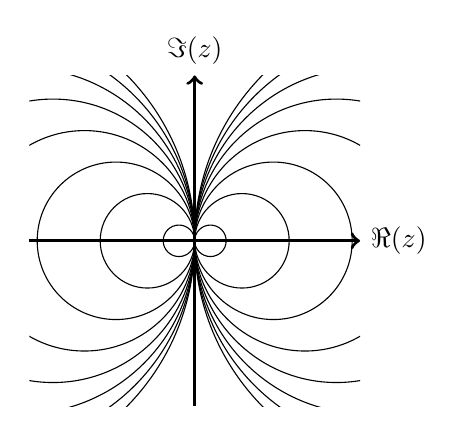
\begin{tikzpicture}[scale=0.2]
  % die Koordinatenachsen
  \draw[very thick,->] (-10.5,0) -- (10.5,0) node[anchor=west] {$\Re(z)$}; % Re-Achse
  \draw[very thick,->] (0,-10.5) -- (0,10.5) node[anchor=south] {$\Im(z)$}; % Im-Achse
  % Niveulinien
  \begin{scope}
   \clip (-10.5,-10.5) rectangle (10.5,10.5);
   \foreach \r in {-15, -13, ..., 13, 15}
    \draw (\r,0) circle (\r);
  \end{scope}
 \end{tikzpicture}
 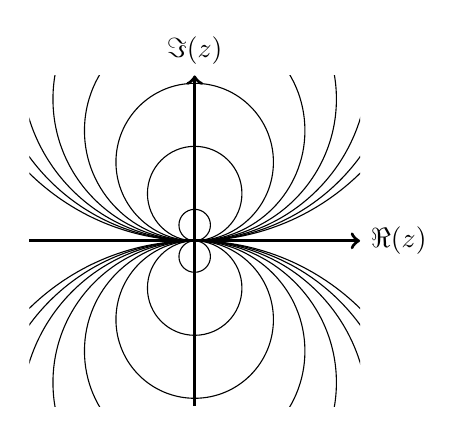
\begin{tikzpicture}[scale=0.2]
  % die Koordinatenachsen
  \draw[very thick,->] (-10.5,0) -- (10.5,0) node[anchor=west] {$\Re(z)$}; % Re-Achse
  \draw[very thick,->] (0,-10.5) -- (0,10.5) node[anchor=south] {$\Im(z)$}; % Im-Achse
  % Niveulinien
  \begin{scope}
   \clip (-10.5,-10.5) rectangle (10.5,10.5);
   \foreach \r in {-15, -13, ..., 13, 15}
    \draw (0,\r) circle (\r);
  \end{scope}
 \end{tikzpicture}
 \caption{Niveulinien von $\Re(1/z)$ und $\Im(1/z)$.}
 \label{fig: Niveulinien von 1/z}
\end{figure}















\section{(Real- und Imaginärteil quadratischer Funktionen)}
Wir behaupten, dass $p(x,y) = ax^2 + bxy + cy^2$ mit $a,b,c \in \R$ genau dann Realteil des komplexen Polynoms $P(z) = Az^2 + Bz + C$ ist, wenn $c = -a$.

Ist $c = -a$, so ist für beliebiges $b \in \R$
\[
 p(x,y) = ax^2 + bxy - ay^2 = \Re\left(\left(a-\frac{1}{2}bi\right)(x+iy)^2\right).
\]

Sei andererseits $p = \Re(P)$. Da
\[
 \Re(C) = \Re(P(0)) = p(0,0) = 0
\]
ist $p = \Re(Az^2+Bz)$, wir können also o.B.d.A. davon ausgehen, dass $C=0$. Da für alle $z = x+iy \in \C$
\begin{align*}
 0 &= p(x,y) - p(-x,-y) = \Re(P(z))-\Re(P(-z)) \\
   &= \Re(P(z)-P(-z)) = \Re(Bz - B(-z)) = \Re(2Bz) = 2 \Re(Bz)
\end{align*}
ist $\Re(Bz) = 0$ für alle $z \in \C$. Da $0 = \Re(B \bar{B}) = \Re(|B|^2)= |B|^2$ folgt daraus, dass $B = 0$. Also ist $P(z) = Az^2$ für $A = x_A + iy_A \in \C$. Es ist daher
\[
 p(x,y) = \Re(Az^2) = \Re((x_A+iy_A)(x+iy)^2) = x_Ax^2 - 2y_Axy - x_A y^2,
\]
was die Behauptung zeigt.

Man bemerke noch, dass $p$ genau dann Imaginärteil eines komplexen Polynoms vom Grad $n$ ist, wenn $p$ Realteil eines komplexen Polynoms vom Grad $n$ ist, denn $p = \Im(P) \Leftrightarrow p = \Re(-iP)$, bzw. $p = \Re(P) \Leftrightarrow p = \Im(iP)$ für jedes komplexe Polynom $P$. Also ist $p$ genau dann Imaginärteil eines Polynoms $P(z) = Az^2+Bz+C$, wenn $a = -c$.





\section{Betrag der Exponentialabbildung}
Für alle $z \in \C$ ist
\[
 |e^z| = \left|e^{\Re(z)+i\Im(z)}\right| = \left|e^{\Re(z)} e^{i\Im(z)}\right|
 = \left|e^{\Re(z)}\right| \left|e^{i\Im(z)}\right| = e^{\Re(z)}.
\]













\end{document}
